\section{Durchführung}
\label{sec:Durchführung}
Für diesen Versuch wird ein Aufbau verwendet, der in \autoref{fig:Aufbau} zu sehen ist.
\begin{figure}[H]
    \centering
    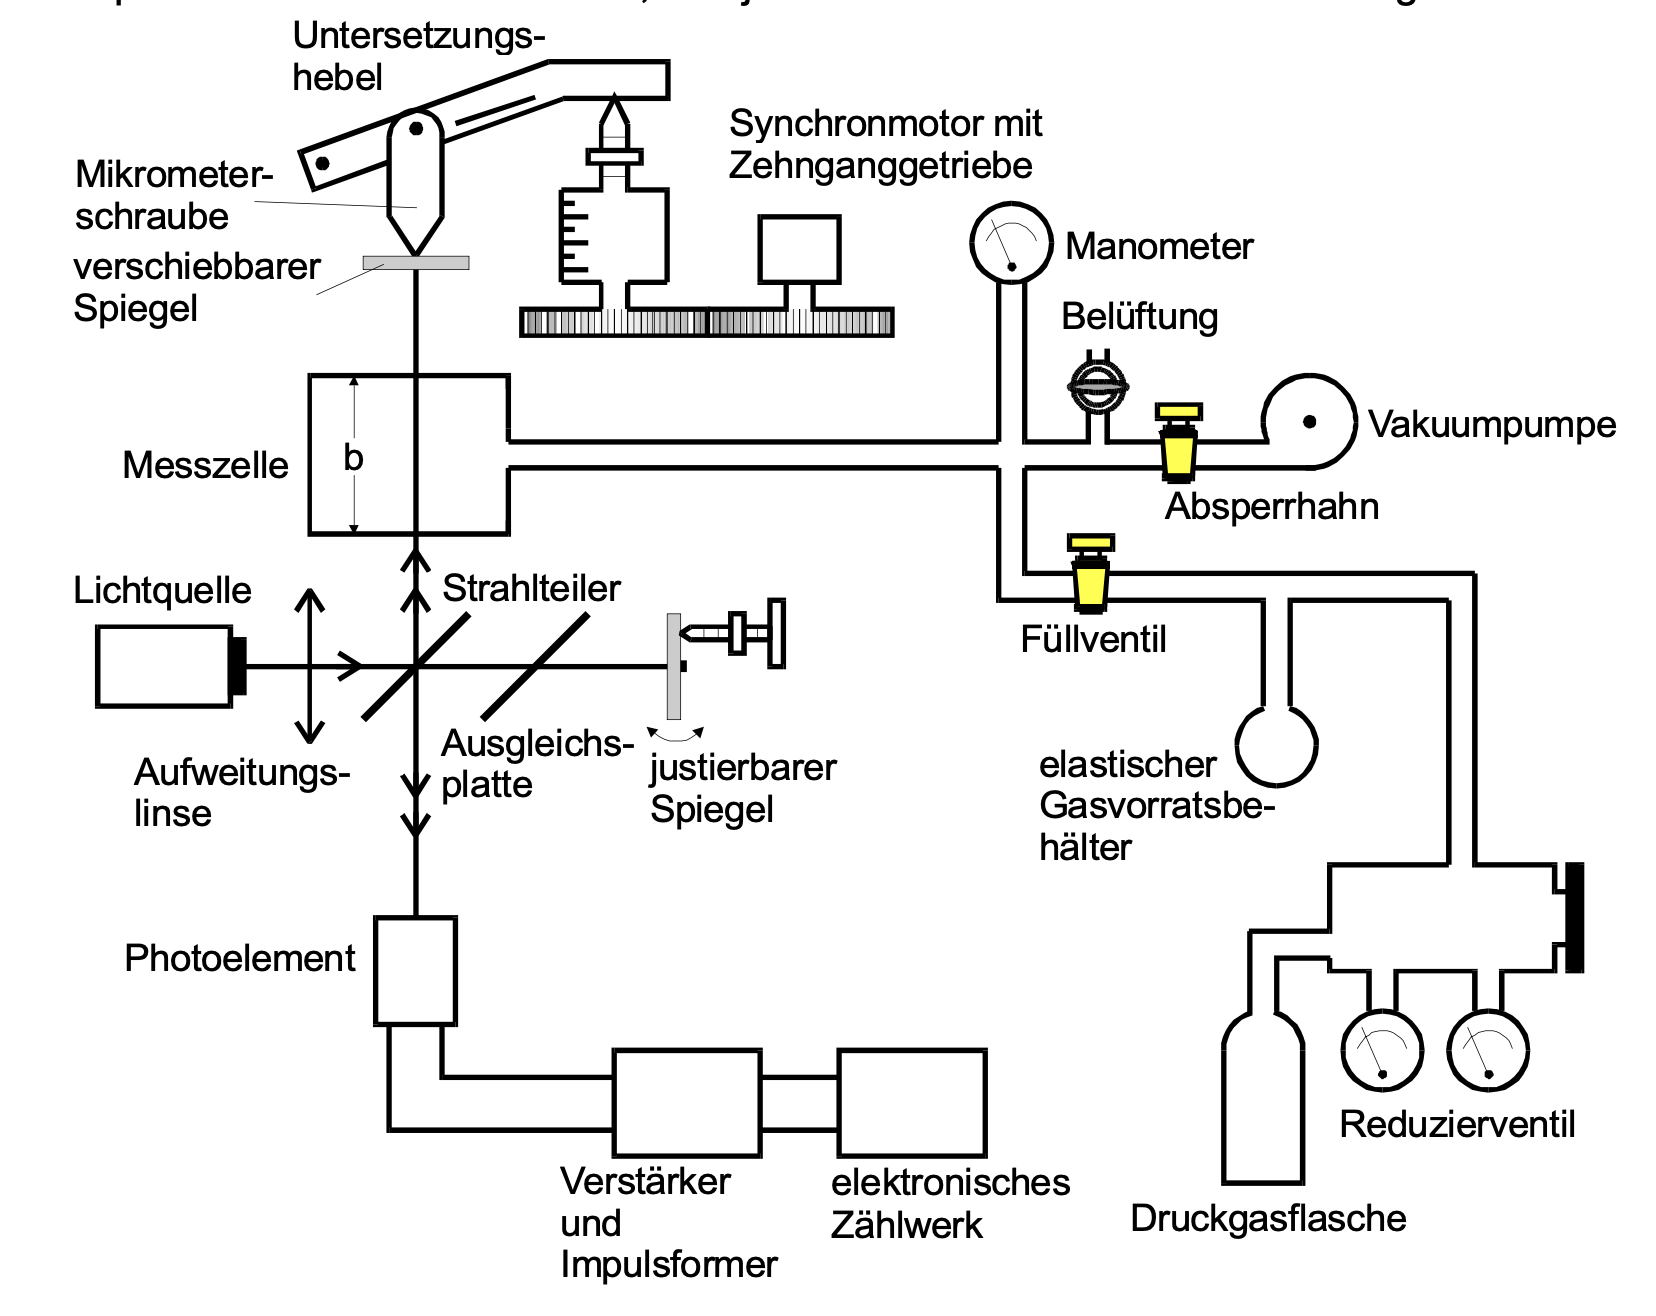
\includegraphics[height=7cm]{content/pics/Aufbau.png}
    \caption{Skizze des Versuchaufbaus \cite{v401}.}
    \label{fig:Aufbau}
  \end{figure}
Bevor die eigentlichen Messungen starten, wird mithilfe der Stellschrauben am justierbaren Spiegel die Überlagerung
der Strahlen so eingestellt, dass diese möglichst exakt übereinander liegen und die Intersitätsextrema breit sind.

Über den Synchronmotor lässt sich die Entfernung des anderen Spiegels verstellen und die Photokathode regisitert die
Maxima und Minima.